% ==========================================
% 第一章:绪论
% ==========================================

\chapter{绪论}
\label{chap:introduction}

% 问题驱动开篇
如何让机器学会下棋?监督学习的做法是给机器看大量棋谱,模仿人类高手的落子。但这有两个问题:一是棋谱覆盖不了所有可能的局面;二是下棋是\textbf{序列决策}——当前这步棋的好坏,可能要几十步后才能评判。

强化学习(Reinforcement Learning, RL)解决的正是这类问题:agent(智能体)通过与环境交互,在没有"标准答案"的情况下,逐渐学会做出最优决策。

本章的目标是建立 RL 的数学框架,核心结论是:RL 问题可以形式化为 Markov Decision Process(MDP),目标是找到使期望累积奖励最大的策略。

% ------------------------------------------
\section{强化学习概述}
\label{sec:rl-overview}

\subsection{什么是强化学习}

强化学习是机器学习的一个重要分支,研究 agent 如何通过与环境的交互来学习最优决策策略。与监督学习和无监督学习相比,RL 有三个显著特点:

\begin{itemize}
    \item \textbf{交互式学习}:Agent 通过执行动作、观察反馈来积累经验,没有"正确答案"的标签
    \item \textbf{延迟奖励}:动作的好坏可能要很久之后才能知道(想想下棋时的"弃子争先")
    \item \textbf{序列决策}:当前决策影响未来状态,数据分布由策略自身决定
\end{itemize}

\begin{figure}[H]
    \centering
    \begin{tikzpicture}[scale=1.0, every node/.style={scale=1.0}]
        % Agent box
        \node[draw, rounded corners, fill=blue!10, minimum width=4cm, minimum height=2.5cm] (agent) {};
        \node[above=0.05cm of agent.north] {\textbf{Agent}};
        \node[draw, rounded corners, fill=orange!30, minimum width=2.5cm, minimum height=1cm] at (agent.center) (policy) {策略 $\policy(a|s)$};

        % Environment box
        \node[draw, rounded corners, fill=green!20, minimum width=4cm, minimum height=1.8cm, below=2.5cm of agent] (env) {\textbf{Environment}};

        % Arrows with labels
        \draw[->, very thick, blue!70] (agent.east) -- ++(1.5,0) |- node[right, pos=0.25] {动作 $a_t$} (env.east);
        \draw[->, very thick, red!70] (env.west) -- ++(-1.5,0) |- node[left, pos=0.25] {\begin{tabular}{c}状态 $s_{t+1}$\\奖励 $r_t$\end{tabular}} (agent.west);

        % Time annotation (positioned below Environment box to avoid overlap)
        \node[gray, font=\small, below=0.5cm of env] {时刻 $t$: Agent 观察 $s_t$,执行 $a_t$;环境返回 $r_t$ 和 $s_{t+1}$};
    \end{tikzpicture}
    \caption{Agent-Environment 交互循环。这是 RL 的基本范式:Agent 根据当前状态选择动作,环境根据动作返回奖励和新状态。这个循环不断重复,直到任务结束或无限持续。}
    \label{fig:agent-env-loop}
\end{figure}

\subsection{与监督学习的本质区别}

RL 与监督学习最关键的区别在于\textbf{数据分布}。监督学习假设数据独立同分布(i.i.d.),但 RL 中数据分布完全取决于当前策略——策略一变,采集到的数据就变了。

\begin{table}[H]
    \centering
    \begin{tabular}{@{}lccc@{}}
        \toprule
        \textbf{特性} & \textbf{监督学习} & \textbf{无监督学习} & \textbf{强化学习} \\
        \midrule
        反馈类型 & 标签(正确答案) & 无反馈 & 奖励信号(标量) \\
        数据分布 & i.i.d. & i.i.d. & \textbf{由策略决定,非 i.i.d.} \\
        目标 & 最小化预测误差 & 发现数据结构 & 最大化累积奖励 \\
        决策时序 & 单步独立决策 & 无决策 & 序列相关决策 \\
        \bottomrule
    \end{tabular}
    \caption{三种机器学习范式对比。RL 的核心难点在于数据分布由策略自身决定,导致 distribution shift 问题。}
    \label{tab:ml-comparison}
\end{table}

这个区别带来了实际训练中的诸多困难:策略变化导致数据分布变化,而数据分布变化又影响策略更新,形成复杂的动态过程。

\begin{keypoint}
RL 的三大核心挑战:
\begin{enumerate}
    \item \textbf{探索与利用的权衡}(Exploration vs. Exploitation):应该尝试新动作(探索)还是使用已知好动作(利用)?过度探索浪费资源,过度利用可能错过更好的策略。
    \item \textbf{信用分配问题}(Credit Assignment):最终奖励如何归因到之前的各个动作?在下棋中,哪一步导致了最终的胜利或失败?
    \item \textbf{非稳态性}:数据分布随策略变化而变化,这让训练变得不稳定,也是 RL 比监督学习更难的根本原因。
\end{enumerate}
\end{keypoint}

\subsection{应用场景}

RL 在众多领域取得了突破性进展:

\begin{itemize}
    \item \textbf{游戏 AI}:AlphaGo(围棋)击败世界冠军、OpenAI Five(Dota 2)、AlphaStar(星际争霸)
    \item \textbf{机器人控制}:机械臂精细操作、四足机器人运动、无人机控制
    \item \textbf{自动驾驶}:决策规划、路径规划
    \item \textbf{推荐系统}:优化长期用户满意度而非即时点击率
    \item \textbf{大语言模型对齐}:RLHF(Reinforcement Learning from Human Feedback)已成为 GPT、Claude 等模型的标准训练流程
\end{itemize}

值得注意的是,近年来 RL 最成功的应用可能不是游戏,而是 LLM 对齐——这也是本书第 \ref{chap:llm-rl} 章的重点内容。

% ------------------------------------------
\section{Markov Decision Process (MDP)}
\label{sec:mdp}

有了直观理解后,我们来建立数学框架。MDP 是 RL 的标准形式化工具,它把 agent 与环境的交互过程描述为一个离散时间随机控制过程。

\subsection{MDP 五元组定义}

\begin{definition}[Markov Decision Process]
\label{def:mdp}
一个 MDP 由五元组 $(\statespace, \actionspace, P, R, \discount)$ 定义:
\begin{itemize}
    \item $\statespace$:\textbf{状态空间}(State Space),所有可能状态的集合
    \item $\actionspace$:\textbf{动作空间}(Action Space),所有可能动作的集合
    \item $P: \statespace \times \actionspace \times \statespace \to [0,1]$:\textbf{状态转移概率},$P(s'|s,a)$ 表示在状态 $s$ 执行动作 $a$ 后转移到状态 $s'$ 的概率
    \item $R: \statespace \times \actionspace \to \R$:\textbf{奖励函数},$R(s,a)$ 表示在状态 $s$ 执行动作 $a$ 获得的即时奖励
    \item $\discount \in [0,1]$:\textbf{折扣因子}(Discount Factor),权衡即时奖励与未来奖励的相对重要性
\end{itemize}
\end{definition}

\begin{figure}[H]
    \centering
    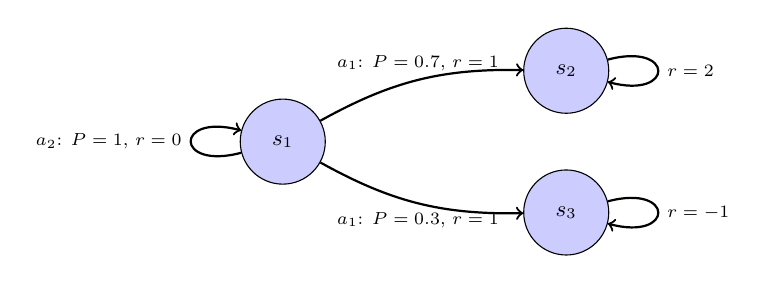
\begin{tikzpicture}[scale=0.9, every node/.style={scale=0.9},
        state/.style={circle, draw, fill=blue!20, minimum size=1.2cm, font=\small},
        action/.style={rectangle, draw, fill=orange!20, minimum width=0.8cm, minimum height=0.6cm, font=\scriptsize}]

        % States
        \node[state] (s1) at (0,0) {$s_1$};
        \node[state] (s2) at (4,1) {$s_2$};
        \node[state] (s3) at (4,-1) {$s_3$};

        % Transitions from s1
        \draw[->, thick, bend left=15] (s1) to node[above, font=\scriptsize] {$a_1$: $P=0.7$, $r=1$} (s2);
        \draw[->, thick, bend right=15] (s1) to node[below, font=\scriptsize] {$a_1$: $P=0.3$, $r=1$} (s3);
        \draw[->, thick] (s1) to[loop left] node[left, font=\scriptsize] {$a_2$: $P=1$, $r=0$} (s1);

        % Self loops
        \draw[->, thick] (s2) to[loop right] node[right, font=\scriptsize] {$r=2$} (s2);
        \draw[->, thick] (s3) to[loop right] node[right, font=\scriptsize] {$r=-1$} (s3);
    \end{tikzpicture}
    \caption{一个简单的 MDP 示例。状态 $s_1$ 有两个动作可选:$a_1$ 以 0.7 概率转移到 $s_2$(高奖励),0.3 概率转移到 $s_3$(负奖励);$a_2$ 原地不动但无奖励。}
    \label{fig:mdp-example}
\end{figure}

\begin{note}
奖励函数的定义有多种形式:
\begin{itemize}
    \item $R(s,a)$:只依赖于当前状态和动作
    \item $R(s,a,s')$:还依赖于下一状态
    \item $R(s)$:只依赖于状态
\end{itemize}
这些形式可以相互转化。例如,$R(s,a,s')$ 可以转化为 $R(s,a) = \sum_{s'} P(s'|s,a) R(s,a,s')$。本书默认使用 $R(s,a)$ 形式。
\end{note}

\subsection{Markov 性质}

MDP 的核心假设是 \textbf{Markov 性质}(Markov Property),也称为"无记忆性":

\begin{definition}[Markov 性质]
\label{def:markov-property}
给定当前状态 $s_t$ 和动作 $a_t$,下一状态 $s_{t+1}$ 和奖励 $r_t$ 的分布只依赖于 $(s_t, a_t)$,与历史状态和动作无关:
\begin{equation}
    P(s_{t+1}, r_t | s_t, a_t) = P(s_{t+1}, r_t | s_0, a_0, s_1, a_1, \ldots, s_t, a_t)
\end{equation}
\end{definition}

直观理解:\textbf{当前状态包含了预测未来所需的所有信息}。历史轨迹可以被"压缩"为当前状态,状态是对历史的"充分统计量"。

\begin{keypoint}
如果真实环境不满足 Markov 性质怎么办?答案是扩展状态表示:
\begin{itemize}
    \item \textbf{历史窗口}:Atari 游戏中用连续 4 帧图像作为状态,捕捉运动信息
    \item \textbf{RNN 隐状态}:用循环神经网络的隐状态编码历史
    \item \textbf{Transformer}:用 attention 机制处理变长历史
\end{itemize}
本质上是把"历史"编码进状态表示里,使得扩展后的状态满足 Markov 性质。
\end{keypoint}

\subsection{状态空间与动作空间的分类}

根据状态空间和动作空间的性质,RL 问题可以分类为:

\begin{table}[H]
    \centering
    \begin{tabular}{@{}lllp{5cm}@{}}
        \toprule
        \textbf{类型} & \textbf{状态空间} & \textbf{动作空间} & \textbf{典型例子} \\
        \midrule
        离散-离散 & 有限/可数 & 有限/可数 & 棋类游戏(棋盘布局 $\times$ 落子位置) \\
        连续-离散 & $\R^n$ & 有限/可数 & Atari 游戏(像素图像 $\times$ 按键) \\
        连续-连续 & $\R^n$ & $\R^m$ & 机器人控制(关节角度 $\times$ 力矩) \\
        \bottomrule
    \end{tabular}
    \caption{RL 问题的分类}
    \label{tab:rl-types}
\end{table}

% ------------------------------------------
\section{轨迹与回报}
\label{sec:trajectory-return}

\subsection{轨迹的定义}

Agent 与环境交互产生的状态-动作-奖励序列称为\textbf{轨迹}(Trajectory),也叫 episode 或 rollout。

\begin{definition}[轨迹]
\label{def:trajectory}
轨迹 $\trajectory$ 是一个状态、动作、奖励的序列:
\begin{equation}
    \trajectory = (s_0, a_0, r_0, s_1, a_1, r_1, \ldots, s_{T-1}, a_{T-1}, r_{T-1}, s_T)
\end{equation}
其中 $T$ 是轨迹的长度(episode 的终止时刻)。
\end{definition}

\begin{figure}[H]
    \centering
    \begin{tikzpicture}[scale=0.85, every node/.style={scale=0.85},
        state/.style={circle, draw, fill=blue!20, minimum size=1.1cm, font=\small},
        action/.style={rectangle, draw, fill=orange!20, minimum size=0.7cm, font=\small}]

        \node[state] (s0) at (0,0) {$s_0$};
        \node[action] (a0) at (2,0) {$a_0$};
        \node[state] (s1) at (4,0) {$s_1$};
        \node[action] (a1) at (6,0) {$a_1$};
        \node[state] (s2) at (8,0) {$s_2$};
        \node[action] (a2) at (10,0) {$a_2$};
        \node at (11.5,0) {$\cdots$};
        \node[state] (sT) at (13,0) {$s_T$};

        % 状态到动作的箭头(策略)
        \draw[->, thick] (s0) -- node[above] {\scriptsize $\policy(a_0|s_0)$} (a0);
        \draw[->, thick] (s1) -- node[above] {\scriptsize $\policy(a_1|s_1)$} (a1);
        \draw[->, thick] (s2) -- node[above] {\scriptsize $\policy(a_2|s_2)$} (a2);

        % 动作到状态的箭头(环境转移),使用 yshift 避免标签重叠
        \draw[->, thick] (a0) -- node[above, yshift=1pt] {\scriptsize $r_0$} node[below, yshift=-8pt] {\scriptsize $P(s_1|s_0,a_0)$} (s1);
        \draw[->, thick] (a1) -- node[above, yshift=1pt] {\scriptsize $r_1$} node[below, yshift=-8pt] {\scriptsize $P(s_2|s_1,a_1)$} (s2);
        \draw[->, thick] (a2) -- node[above] {\scriptsize $r_2$} (11.3,0);
        \draw[->, thick] (11.7,0) -- (sT);

        % Legend - 放在图下方,避免与转移概率标签重叠
        \node[blue!70, font=\footnotesize] at (2, -2.0) {策略决定动作};
        \node[green!50!black, font=\footnotesize] at (7, -2.0) {环境决定转移和奖励};
    \end{tikzpicture}
    \caption{轨迹的生成过程。蓝色圆圈表示状态,橙色方块表示动作。注意两种概率来源:策略 $\policy$ 决定动作,环境 $P$ 决定状态转移。}
    \label{fig:trajectory}
\end{figure}

\subsection{轨迹概率分解}

轨迹的概率如何计算?

\begin{theorem}[轨迹概率分解]
\label{thm:trajectory-prob}
在策略 $\policy$ 下,轨迹 $\trajectory$ 的概率为:
\begin{equation}
    p(\trajectory | \policy) = p(s_0) \prod_{t=0}^{T-1} \policy(a_t | s_t) \cdot P(s_{t+1} | s_t, a_t)
    \label{eq:trajectory-prob}
\end{equation}
\end{theorem}

\begin{proof}
利用条件概率的链式法则和 Markov 性质:
\begin{align}
    p(\trajectory | \policy) &= p(s_0, a_0, s_1, a_1, \ldots, s_T | \policy) \\
    &= p(s_0) \cdot p(a_0 | s_0) \cdot p(s_1 | s_0, a_0) \cdot p(a_1 | s_1) \cdot p(s_2 | s_1, a_1) \cdots \\
    &= p(s_0) \prod_{t=0}^{T-1} \underbrace{p(a_t | s_t)}_{\policy(a_t|s_t)} \cdot \underbrace{p(s_{t+1} | s_t, a_t)}_{P(s_{t+1}|s_t,a_t)}
\end{align}
其中第二步使用了 Markov 性质:$p(s_{t+1} | s_0, a_0, \ldots, s_t, a_t) = p(s_{t+1} | s_t, a_t)$。
\end{proof}

\begin{important}
这个分解非常重要!观察公式 \eqref{eq:trajectory-prob}:
\begin{itemize}
    \item $p(s_0)$:初始状态分布,由环境决定
    \item $\policy(a_t|s_t)$:策略,是我们要学习/优化的对象
    \item $P(s_{t+1}|s_t,a_t)$:环境动力学,由环境决定
\end{itemize}

关键观察:$p(s_0)$ 和 $P(s_{t+1}|s_t,a_t)$ 与策略参数 $\theta$ 无关。因此,当对 $\log p(\trajectory|\policy_\theta)$ 求关于 $\theta$ 的梯度时,环境动力学项会消失!这是 Policy Gradient 定理的核心(见第 \ref{chap:policy-based} 章)。
\end{important}

\subsection{Return(回报)的定义}

\begin{definition}[回报 / Reward-to-go]
\label{def:return}
从时刻 $t$ 开始的\textbf{回报}(Return)或\textbf{Reward-to-go} 定义为未来奖励的折扣累积和:
\begin{equation}
    G_t = \sum_{k=0}^{\infty} \discount^k r_{t+k} = r_t + \discount r_{t+1} + \discount^2 r_{t+2} + \cdots
    \label{eq:return}
\end{equation}
其中 $\discount \in [0,1]$ 是折扣因子。
\end{definition}

回报 $G_t$ 满足一个简单但重要的递推关系:
\begin{equation}
    G_t = r_t + \discount G_{t+1}
    \label{eq:return-recursive}
\end{equation}

Bellman 方程正是基于这个递推结构——下一章将详细展开。

\begin{figure}[H]
    \centering
    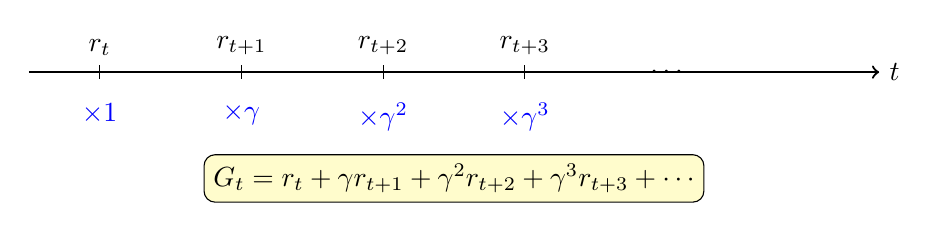
\begin{tikzpicture}[scale=0.9]
        % Timeline
        \draw[->, thick] (0,0) -- (12,0) node[right] {$t$};

        % Rewards
        \foreach \x/\r in {1/$r_t$, 3/$r_{t+1}$, 5/$r_{t+2}$, 7/$r_{t+3}$} {
            \draw (\x, 0.1) -- (\x, -0.1);
            \node[above] at (\x, 0.1) {\r};
        }
        \node at (9, 0) {$\cdots$};

        % Discount factors
        \node[below, blue] at (1, -0.3) {$\times 1$};
        \node[below, blue] at (3, -0.3) {$\times \gamma$};
        \node[below, blue] at (5, -0.3) {$\times \gamma^2$};
        \node[below, blue] at (7, -0.3) {$\times \gamma^3$};

        % G_t
        \node[draw, rounded corners, fill=yellow!20] at (6, -1.5) {$G_t = r_t + \gamma r_{t+1} + \gamma^2 r_{t+2} + \gamma^3 r_{t+3} + \cdots$};
    \end{tikzpicture}
    \caption{回报 $G_t$ 的计算:未来奖励按 $\gamma^k$ 折扣后求和。$\gamma$ 越小,远期奖励的权重越低。}
    \label{fig:return}
\end{figure}

\subsection{Episodic vs Continuing Tasks}

根据任务是否有终止状态,RL 问题分为两类:

\begin{definition}[Episodic 与 Continuing Tasks]\leavevmode
\begin{description}
    \item[Episodic Task] 存在终止状态 $s_T$,轨迹有限长度。例如:棋类游戏(胜负终局)、机器人完成特定任务、一局游戏
    \item[Continuing Task] 没有终止状态,$T \to \infty$。例如:股票交易、持续运行的控制系统、服务器调度
\end{description}
\end{definition}

对于 Continuing Task,必须使用 $\discount < 1$ 以确保回报有界。当 $|r_t| \leq R_{\max}$ 时:
\begin{equation}
    |G_t| \leq \sum_{k=0}^{\infty} \discount^k R_{\max} = \frac{R_{\max}}{1 - \discount}
\end{equation}

\subsection{折扣因子的多重意义}

折扣因子 $\discount$ 是一个看似简单但含义丰富的超参数:

\begin{itemize}
    \item $\discount = 0$:Agent 只关心即时奖励,完全忽略未来("短视")
    \item $\discount = 1$:Agent 平等对待所有未来奖励(仅适用于 Episodic Task)
    \item $0 < \discount < 1$:权衡即时与未来奖励,$\discount$ 越大越"远视"
\end{itemize}

\begin{keypoint}
折扣因子的多重理解:
\begin{enumerate}
    \item \textbf{数学角度}:确保无限和收敛,$G_t$ 有界
    \item \textbf{经济学角度}:时间价值——"现在的 1 元比未来的 1 元更值钱"
    \item \textbf{不确定性角度}:未来越远,预测越不准确,应降低权重
    \item \textbf{实践角度}:$\discount$ 定义了"有效时间尺度"。$1/(1-\discount)$ 步之外的奖励贡献会指数衰减到可以忽略。例如 $\discount=0.99$ 时,有效视野约 100 步。
\end{enumerate}
\end{keypoint}

% ------------------------------------------
\section{策略与价值函数}
\label{sec:policy-value}

\subsection{策略的定义}

\begin{definition}[策略]
\label{def:policy}
\textbf{策略}(Policy)$\policy$ 是从状态到动作的映射,定义了 agent 在每个状态下如何选择动作。策略分为两类:
\begin{itemize}
    \item \textbf{确定性策略}(Deterministic Policy):$\policy: \statespace \to \actionspace$,即 $a = \policy(s)$
    \item \textbf{随机策略}(Stochastic Policy):$\policy: \statespace \times \actionspace \to [0,1]$,即 $\policy(a|s)$ 表示在状态 $s$ 选择动作 $a$ 的概率
\end{itemize}
\end{definition}

随机策略满足归一化条件:对于所有 $s \in \statespace$,
\begin{equation}
    \sum_{a \in \actionspace} \policy(a|s) = 1
\end{equation}

为什么需要随机策略?确定性策略不是更简单吗?

\begin{note}
随机策略的三个优势:
\begin{enumerate}
    \item \textbf{探索}:随机性有助于探索未知动作,避免陷入局部最优
    \item \textbf{对抗性}:在博弈场景中,确定性策略容易被对手预测(想想"石头剪刀布")
    \item \textbf{优化友好}:随机策略的梯度更容易计算(确定性策略的梯度涉及 $\argmax$,不可微)
\end{enumerate}
确定性策略可以看作随机策略的特例(概率集中在单一动作上)。
\end{note}

\subsection{状态价值函数 $\Val^\policy(s)$}

\begin{definition}[状态价值函数]
\label{def:state-value}
策略 $\policy$ 的\textbf{状态价值函数}(State Value Function)定义为从状态 $s$ 出发,遵循策略 $\policy$ 的期望回报:
\begin{equation}
    \Val^\policy(s) = \E_\policy \left[ G_t \mid S_t = s \right] = \E_\policy \left[ \sum_{k=0}^{\infty} \discount^k r_{t+k} \mid S_t = s \right]
    \label{eq:state-value}
\end{equation}
其中期望是对策略 $\policy$ 下产生的所有可能轨迹取的。
\end{definition}

$\Val^\policy(s)$ 回答的问题是:\textbf{在状态 $s$,如果从现在开始一直遵循策略 $\policy$,能获得的期望总奖励是多少?}

\subsection{动作价值函数 $\Qval^\policy(s,a)$}

\begin{definition}[动作价值函数]
\label{def:action-value}
策略 $\policy$ 的\textbf{动作价值函数}(Action Value Function)定义为在状态 $s$ 执行动作 $a$,之后遵循策略 $\policy$ 的期望回报:
\begin{equation}
    \Qval^\policy(s,a) = \E_\policy \left[ G_t \mid S_t = s, A_t = a \right] = \E_\policy \left[ \sum_{k=0}^{\infty} \discount^k r_{t+k} \mid S_t = s, A_t = a \right]
    \label{eq:action-value}
\end{equation}
\end{definition}

$\Qval^\policy(s,a)$ 比 $\Val^\policy(s)$ 提供了更细粒度的信息:它允许我们单独评估每个动作的价值,而不是只知道"按 $\policy$ 走的整体期望"。这使得我们可以比较不同动作的好坏,从而改进策略。

\subsection{$\Val$ 与 $\Qval$ 的关系}

两个价值函数之间存在简单而重要的联系:

\begin{theorem}[$\Val$ 与 $\Qval$ 的关系]
\label{thm:v-q-relation}
\begin{equation}
    \Val^\policy(s) = \sum_{a \in \actionspace} \policy(a|s) \Qval^\policy(s,a) = \E_{a \sim \policy(\cdot|s)} \left[ \Qval^\policy(s,a) \right]
    \label{eq:v-from-q}
\end{equation}
\end{theorem}

\begin{proof}
由全期望公式:
\begin{align}
    \Val^\policy(s) &= \E_\policy \left[ G_t \mid S_t = s \right] \\
    &= \sum_{a \in \actionspace} p(A_t = a | S_t = s) \cdot \E_\policy \left[ G_t \mid S_t = s, A_t = a \right] \\
    &= \sum_{a \in \actionspace} \policy(a|s) \cdot \Qval^\policy(s,a)
\end{align}
\end{proof}

直观理解:状态价值 $\Val^\policy(s)$ 就是所有动作价值 $\Qval^\policy(s,a)$ 按策略概率 $\policy(a|s)$ 加权的平均。

\subsection{优势函数 $\advantage^\policy(s,a)$}

\begin{definition}[优势函数]
\label{def:advantage}
\textbf{优势函数}(Advantage Function)定义为动作价值与状态价值之差:
\begin{equation}
    \advantage^\policy(s,a) = \Qval^\policy(s,a) - \Val^\policy(s)
    \label{eq:advantage}
\end{equation}
\end{definition}

优势函数衡量的是:在状态 $s$ 执行动作 $a$ 相对于"平均水平"(即按策略采样动作)好多少或差多少。

\begin{theorem}[优势函数的关键性质]
\label{thm:advantage-properties}
优势函数在策略分布下的期望为零:
\begin{equation}
    \E_{a \sim \policy(\cdot|s)} \left[ \advantage^\policy(s,a) \right] = 0
\end{equation}
\end{theorem}

\begin{proof}
由公式 \eqref{eq:v-from-q}:
\begin{align}
    \E_{a \sim \policy(\cdot|s)} \left[ \advantage^\policy(s,a) \right]
    &= \E_{a \sim \policy} \left[ \Qval^\policy(s,a) - \Val^\policy(s) \right] \\
    &= \E_{a \sim \policy} \left[ \Qval^\policy(s,a) \right] - \Val^\policy(s) \\
    &= \Val^\policy(s) - \Val^\policy(s) = 0
\end{align}
\end{proof}

\begin{keypoint}
优势函数的直观意义:
\begin{itemize}
    \item $\advantage(s,a) > 0$:动作 $a$ 优于平均水平
    \item $\advantage(s,a) < 0$:动作 $a$ 劣于平均水平
    \item $\advantage(s,a) = 0$:动作 $a$ 与平均水平持平
\end{itemize}
优势函数在 Policy Gradient 中的作用将在第~\ref{chap:policy-based}~章详细讨论。
\end{keypoint}

\subsection{最优策略与最优价值函数}

\begin{definition}[最优价值函数]
\label{def:optimal-value}
\textbf{最优状态价值函数} $\Val^*(s)$ 和\textbf{最优动作价值函数} $\Qval^*(s,a)$ 定义为所有策略中能达到的最大价值:
\begin{align}
    \Val^*(s) &= \max_\policy \Val^\policy(s) \label{eq:optimal-v} \\
    \Qval^*(s,a) &= \max_\policy \Qval^\policy(s,a) \label{eq:optimal-q}
\end{align}
\end{definition}

\begin{definition}[最优策略]
\label{def:optimal-policy}
策略 $\policy^*$ 称为\textbf{最优策略}(Optimal Policy),如果对于所有状态 $s \in \statespace$:
\begin{equation}
    \Val^{\policy^*}(s) = \Val^*(s)
\end{equation}
\end{definition}

\begin{theorem}[最优策略的存在性]
对于有限 MDP(有限状态空间和动作空间),至少存在一个确定性最优策略。
\end{theorem}

最优策略可以由最优动作价值函数直接导出:

\begin{theorem}[从 $\Qval^*$ 导出最优策略]
\label{thm:optimal-policy-from-q}
给定 $\Qval^*$,最优策略为:
\begin{equation}
    \policy^*(s) = \argmax_{a \in \actionspace} \Qval^*(s,a)
    \label{eq:optimal-policy-from-q}
\end{equation}
\end{theorem}

这个结论是 Q-Learning 等 Value-Based 方法的理论基础:\textbf{只要学到 $\Qval^*$,就能直接得到最优策略}。

% ------------------------------------------
\section{RL 问题的形式化目标}
\label{sec:rl-objective}

综合以上定义,强化学习的目标可以形式化为:

\begin{definition}[RL 目标]
\label{def:rl-objective}
找到最优策略 $\policy^*$,使得期望回报最大化:
\begin{equation}
    \policy^* = \argmax_\policy J(\policy)
    \label{eq:rl-objective}
\end{equation}
其中 $J(\policy)$ 是策略的性能指标,常见定义包括:
\begin{enumerate}
    \item \textbf{从固定初始状态出发}:$J(\policy) = \Val^\policy(s_0)$
    \item \textbf{初始状态有分布}:$J(\policy) = \E_{s_0 \sim p(s_0)} \left[ \Val^\policy(s_0) \right]$
    \item \textbf{轨迹期望}:$J(\policy) = \E_{\trajectory \sim \policy} \left[ \sum_{t=0}^{T} \discount^t r_t \right]$
\end{enumerate}
\end{definition}

这三种定义在大多数情况下是等价的。后续章节将介绍解决这一优化问题的不同方法:

\begin{itemize}
    \item \textbf{Value-Based 方法}(第 \ref{chap:value-based} 章):学习 $\Val^*$ 或 $\Qval^*$,再由 $\argmax$ 导出 $\policy^*$
    \item \textbf{Policy-Based 方法}(第 \ref{chap:policy-based} 章):直接优化参数化策略 $\policy_\theta$
    \item \textbf{Actor-Critic 方法}(第 \ref{chap:policy-based} 章):同时学习策略(Actor)和价值函数(Critic)
\end{itemize}

\begin{figure}[H]
    \centering
    \begin{tikzpicture}[scale=0.9, every node/.style={scale=0.9},
        box/.style={draw, rounded corners, minimum width=2.8cm, minimum height=1cm, align=center}]

        \node[box, fill=blue!15] (rl) at (0, 0) {RL 方法};

        \node[box, fill=orange!15] (vb) at (-3.5, -2) {Value-Based\\学习 $\Qval^*$};
        \node[box, fill=green!15] (pb) at (0, -2) {Policy-Based\\学习 $\policy_\theta$};
        \node[box, fill=purple!15] (ac) at (3.5, -2) {Actor-Critic\\学习两者};

        \draw[->, thick] (rl) -- (vb);
        \draw[->, thick] (rl) -- (pb);
        \draw[->, thick] (rl) -- (ac);

        \node[font=\scriptsize, gray] at (-3.5, -3.2) {DQN, Q-Learning};
        \node[font=\scriptsize, gray] at (0, -3.2) {REINFORCE, TRPO};
        \node[font=\scriptsize, gray] at (3.5, -3.2) {A2C, PPO, SAC};
    \end{tikzpicture}
    \caption{RL 方法的三大类别。Value-Based 学习价值函数,Policy-Based 直接学习策略,Actor-Critic 结合两者。}
    \label{fig:rl-methods}
\end{figure}

% ------------------------------------------
\section*{本章小结}

\begin{keypoint}
回顾开篇问题:如何让机器学会序列决策?答案是将问题形式化为 MDP,目标是最大化期望累积奖励。

本章建立的核心概念:
\begin{enumerate}
    \item \textbf{MDP 五元组} $(\statespace, \actionspace, P, R, \discount)$ 是 RL 的标准形式化框架
    \item \textbf{Markov 性质}:当前状态包含预测未来所需的所有信息
    \item \textbf{轨迹概率分解}:$p(\tau|\policy) = p(s_0) \prod_t \policy(a_t|s_t) P(s_{t+1}|s_t,a_t)$,策略与环境动力学分离
    \item \textbf{回报的递推}:$G_t = r_t + \gamma G_{t+1}$,这是 Bellman 方程的起点
    \item \textbf{价值函数}:$\Val^\policy$ 和 $\Qval^\policy$ 衡量策略的长期价值
    \item \textbf{优势函数}:$\advantage^\policy(s,a) = \Qval^\policy(s,a) - \Val^\policy(s)$,期望为零
    \item \textbf{RL 目标}:$\max_\policy J(\policy)$,找到使期望回报最大的策略
\end{enumerate}

下一章将介绍 Bellman 方程——利用回报的递推结构来高效计算价值函数,以及基于价值函数的 Q-Learning、DQN 等算法。
\end{keypoint}

